\chapter{Analyse et conception}
\label{chap:conception}

\section{Analyse des besoins}

\subsection{Besoins fonctionnels}

Le langage \ilang{} et son interpréteur doivent offrir les fonctionnalités
suivantes, directement issues du cahier des charges.

\begin{description}[style=nextline,leftmargin=1em]
  \item[Types de données.] Entiers (seul type initialement requis) ; les booléens
        sont encodés en entiers (0 = faux, tout le reste = vrai), à la manière du
        C.
  \item[Variables.] Déclaration implicite à la première affectation, sans
        mot-clé. Portée globale pour le programme principal, locale pour les
        fonctions.
  \item[Expressions arithmétiques.] Opérateurs \code{+ - * / \%}, moins unaire,
        parenthèses, avec priorité et associativité correctes.
  \item[Comparaisons.] \code{== != < > <= >=}, renvoyant 0 ou 1.
  \item[Structures de contrôle.] Conditionnelle \code{si/sinon}, boucles
        \code{tant que} et \code{pour}.
  \item[Fonctions.] Déclaration avec \code{fonction}, paramètres, valeur de
        retour via \code{retourner}, appels récursifs.
  \item[Entrées-sorties.] \code{afficher(expr)} et \code{lire()}.
  \item[Commentaires.] De ligne (\code{//}) et de bloc (\code{/* */}).
\end{description}

\subsection{Besoins non-fonctionnels}

\begin{description}[style=nextline,leftmargin=1em]
  \item[Correction.] L'interpréteur doit produire les résultats attendus sur les
        programmes de démonstration et gérer proprement les erreurs.
  \item[Robustesse.] Aucune entrée, même fautive, ne doit provoquer de
        comportement indéfini silencieux ; les erreurs sont signalées et
        localisées.
  \item[Qualité du code.] Compilation sans avertissement (\code{-Wall -Wextra}),
        sans conflit grammatical, sans fuite mémoire.
  \item[Portabilité.] Code C standard, compilable sur toute plateforme POSIX
        disposant de GCC, Flex et Bison.
  \item[Lisibilité et maintenabilité.] Découpage en modules à responsabilité
        unique, code commenté.
\end{description}

\subsection{Cas d'utilisation}

L'acteur unique est l'utilisateur (ici, le développeur de programmes \ilang). Les
cas d'utilisation principaux sont : (1)~exécuter un fichier source
(\code{./ilang prog.ilang}) ; (2)~saisir un programme au clavier en mode
interactif (\code{./ilang}) ; (3)~en extension, produire l'assembleur
correspondant (\code{./ilang -s prog.ilang}). Dans tous les cas, le programme lit
le code source, le traduit, l'exécute (ou le compile), et restitue les résultats
ou les messages d'erreur. La figure~\ref{fig:usecase} en donne la vue « cas
d'utilisation ».

\begin{figure}[ht]
\centering
\begin{tikzpicture}[font=\small,
  uc/.style={draw,ellipse,align=center,minimum width=32mm,inner sep=2pt}]
  \node (act) at (0,0) {\begin{tikzpicture}
      \draw (0,0) circle (2.2mm);
      \draw (0,-2.2mm) -- (0,-9mm);
      \draw (-3mm,-5mm) -- (3mm,-5mm);
      \draw (0,-9mm) -- (-3mm,-14mm);
      \draw (0,-9mm) -- (3mm,-14mm);
    \end{tikzpicture}};
  \node[below=8mm of act,font=\footnotesize] {Utilisateur};
  \node[uc] (u1) at (4.5,1.6) {Exécuter un\\fichier \code{.ilang}};
  \node[uc] (u2) at (4.5,0)   {Saisir en mode\\interactif};
  \node[uc] (u3) at (4.5,-1.6){Générer\\l'assembleur};
  \draw (act) -- (u1);
  \draw (act) -- (u2);
  \draw (act) -- (u3);
  \begin{scope}[on background layer]
    \node[draw,dashed,fit=(u1)(u2)(u3),inner sep=4mm,label=above:{\footnotesize Interpréteur \ilang}] {};
  \end{scope}
\end{tikzpicture}
\caption{Diagramme des cas d'utilisation.}
\label{fig:usecase}
\end{figure}

\paragraph{Un programme \ilang{} complet.} Pour fixer les idées, voici un
programme exerçant la plupart des constructions du langage, à savoir une fonction
récursive, une conditionnelle, une boucle et un affichage :

\begin{lstlisting}[style=ilang,caption={Exemple : factorielle récursive et boucle d'affichage.}]
fonction factorielle(n) {
    si (n <= 1) {
        retourner(1)
    }
    retourner(n * factorielle(n - 1))   // appel recursif
}

pour (i = 1; i < 6; i = i + 1) {
    afficher(factorielle(i))            // affiche 1, 2, 6, 24, 120
}
\end{lstlisting}

Ce programme combine déclaration de fonction, récursion, structure
conditionnelle, boucle \code{pour} et entrée-sortie : il servira de fil
conducteur dans la suite du rapport.

\section{Conception architecturale}

\subsection{La chaîne de traitement}

L'architecture suit le modèle classique d'un \emph{pipeline} de compilation, où la
sortie de chaque étage est l'entrée du suivant. La
figure~\ref{fig:pipeline} en donne la vue d'ensemble.

\begin{figure}[ht]
\centering
\begin{tikzpicture}[
  node distance=8mm and 12mm,
  box/.style={draw,rounded corners,minimum height=9mm,minimum width=20mm,align=center,font=\small},
  data/.style={font=\small\itshape,align=center},
  arr/.style={-{Stealth}, very thick}
]
\node[data] (src) {source\\\code{.ilang}};
\node[box,right=of src] (lex) {Flex\\(lexer)};
\node[data,right=of lex] (tok) {tokens};
\node[box,right=of tok] (par) {Bison\\(parseur)};
\node[box,below=of par] (opt) {\code{optim.c}\\(AST $\to$ AST)};
\node[box,left=of opt] (eval) {\code{eval.c}\\(évaluateur)};
\node[data,left=of eval] (res) {résultat};

\draw[arr] (src) -- (lex);
\draw[arr] (lex) -- (tok);
\draw[arr] (tok) -- (par);
\draw[arr] (par) -- node[right,font=\scriptsize]{AST} (opt);
\draw[arr] (opt) -- node[above,font=\scriptsize]{AST optimisé} (eval);
\draw[arr] (eval) -- (res);

\node[box,below=14mm of eval,fill=black!5] (cg) {\code{codegen.c}\\(back-end asm)};
\draw[arr,dashed] (opt.south) |- (cg.east) node[pos=0.25,right,font=\scriptsize]{extension};
\node[data,left=of cg] (asm) {\code{.s} i386};
\draw[arr,dashed] (cg) -- (asm);
\end{tikzpicture}
\caption{Chaîne de traitement d'\ilang. Le front-end (Flex, Bison) est commun ;
seul le back-end diffère entre l'interprétation et la génération de code.}
\label{fig:pipeline}
\end{figure}

\subsection{Patrons de conception (\emph{patterns})}

Deux patrons structurent le logiciel.

\begin{itemize}
  \item \textbf{Pipeline} (chaîne de responsabilité) : chaque module transforme
        une représentation en une autre (texte $\to$ tokens $\to$ AST $\to$ AST
        optimisé $\to$ valeur). Cette séparation rend chaque étage testable et
        remplaçable indépendamment.
  \item \textbf{Parcours d'arbre type \emph{visiteur}} : l'évaluateur, l'optimiseur
        et le générateur de code sont trois « visiteurs » distincts du même AST.
        En C, sans classes, le patron se concrétise par une fonction récursive qui
        distribue (\code{switch}) sur le type du n\oe ud. C'est cette uniformité
        qui a rendu l'ajout du back-end assembleur peu coûteux : un troisième
        visiteur, sans toucher aux deux autres.
\end{itemize}

\subsection{Choix du langage d'implémentation}

L'interpréteur est écrit en \textbf{C}. Ce choix n'est pas neutre et se justifie :

\begin{enumerate}
  \item Flex et Bison génèrent du code C ; écrire le reste en C évite toute
        couche d'interfaçage entre langages.
  \item Le C impose de gérer explicitement la mémoire et les structures de
        données, ce qui est exactement l'objet du cours (pile d'appels, n\oe uds
        alloués dynamiquement).
  \item Le back-end assembleur produit du code 32~bits lié à la \emph{libc} C ;
        rester en C garantit une intégration naturelle.
\end{enumerate}

\subsection{Justification des principales décisions de conception}

Plusieurs décisions de conception méritent d'être explicitées, car à chaque fois
une autre solution était envisageable et le choix retenu résulte d'un arbitrage
que je veux assumer.

La première décision est de construire un arbre syntaxique abstrait plutôt que
d'évaluer le programme directement pendant l'analyse syntaxique. Cette seconde
option, appelée évaluation dirigée par la syntaxe, est parfaitement possible pour
une calculatrice : chaque règle de la grammaire calcule immédiatement sa valeur.
Je l'ai écartée pour une raison de fond. Évaluer pendant l'analyse couplerait
définitivement la syntaxe et la sémantique, interdirait toute passe
d'optimisation, qui suppose de disposer du programme entier avant de l'exécuter,
et rendrait impossible la réutilisation du même travail d'analyse pour produire du
code. En matérialisant le programme sous forme d'arbre, je me donne au contraire
la liberté de le parcourir autant de fois que nécessaire et de plusieurs manières.
C'est exactement cette liberté qui m'a permis, plus tard, d'ajouter un optimiseur
puis un générateur de code sans rien changer à l'analyse.

La deuxième décision concerne la table des symboles. J'aurais pu me contenter
d'une unique table globale, ce qui aurait été plus simple, mais cela aurait rendu
impossible la gestion correcte de la portée locale et de la récursion : deux
appels simultanés de la même fonction auraient partagé les mêmes variables. À
l'inverse, une structure trop élaborée aurait été disproportionnée. La pile
d'environnements, où chaque appel dispose de son propre cadre, est la structure
qui correspond exactement au besoin, et elle a en outre le mérite de reproduire
fidèlement la pile d'appels matérielle étudiée au chapitre~2. Le choix d'une table
de hachage à l'intérieur de chaque cadre, plutôt qu'une simple liste chaînée, vise
la rapidité de recherche : l'accès à une variable est l'opération la plus fréquente
de tout l'évaluateur, et il doit rester proche du temps constant.

La troisième décision, introduite avec l'extension des flottants, est de
représenter une valeur par une union étiquetée distinguant entier et flottant,
plutôt que de tout convertir en flottant. Cette dernière solution aurait été plus
courte à écrire, mais elle aurait silencieusement détruit la sémantique entière
d'origine, en particulier la division entière et le modulo dont dépend le calcul
du PGCD. L'union étiquetée coûte quelques lignes de plus à chaque opération, mais
elle préserve exactement le comportement attendu, ce qui était une contrainte non
négociable de non-régression.

La quatrième décision concerne la gestion des ruptures de flot, c'est-à-dire le
retour de fonction et les instructions \code{arrêter} et \code{continuer}. J'aurais
pu employer les sauts non locaux du C, à savoir \code{setjmp} et \code{longjmp},
ou faire remonter un code de statut par chaque appel de la fonction d'évaluation.
J'ai préféré des indicateurs globaux que les blocs et les boucles consultent. Ce
choix privilégie la lisibilité : le mécanisme tient en quelques lignes et reste
facile à suivre, ce qui compte davantage qu'une élégance théorique dans un
interpréteur mono-thread. J'assume que cette solution introduit un état global,
et j'en discute les limites au chapitre~\ref{chap:discussion}.

\section{Méthodologie et planification}

\subsection{Méthodologie retenue}

Le développement a suivi une démarche \textbf{incrémentale et pilotée par les
tests}. Plutôt que de tout écrire avant d'exécuter quoi que ce soit, le c\oe ur
(entiers seulement) a d'abord été rendu fonctionnel de bout en bout, validé sur
les programmes de démonstration, puis enrichi par étapes (optimisations, puis
extensions, puis back-end). Chaque ajout était suivi d'une vérification de
non-régression. Cette stratégie « marcher avant de courir » s'est révélée
payante : le passage délicat des entiers aux flottants, par exemple, aurait été
bien plus risqué sur une base non encore éprouvée.

\subsection{Identification des tâches et planning}

Le projet se décompose en huit grandes tâches, présentées sous forme de diagramme
de Gantt (figure~\ref{fig:gantt}). Chacune est développée dans la suite du
rapport.

\begin{figure}[ht]
\centering
\resizebox{\textwidth}{!}{%
\begin{ganttchart}[
  vgrid, hgrid,
  bar/.append style={fill=black!25},
  bar incomplete/.append style={fill=black!10},
  group/.append style={fill=black!55},
  title label font=\scriptsize,
  bar label font=\small,
  group label font=\small\bfseries,
  milestone label font=\scriptsize\itshape
]{1}{12}
  \gantttitle{Déroulement du projet (unités de temps relatives)}{12} \\
  \gantttitlelist{1,...,12}{1} \\
  \ganttgroup{Conception}{1}{2} \\
  \ganttbar{Grammaire \& tokens}{1}{2} \\
  \ganttgroup{C\oe ur de l'interpréteur}{2}{6} \\
  \ganttbar{Lexer (Flex)}{2}{3} \\
  \ganttbar{Parseur \& AST (Bison)}{3}{4} \\
  \ganttbar{Évaluateur}{4}{5} \\
  \ganttbar{Table des symboles}{5}{6} \\
  \ganttbar{Optimisations}{6}{6} \\
  \ganttgroup{Tests \& débogage}{5}{8} \\
  \ganttbar{Programmes de démo}{5}{6} \\
  \ganttbar{Gestion des erreurs}{6}{7} \\
  \ganttbar{Vérification (Valgrind)}{7}{8} \\
  \ganttgroup{Extensions}{8}{10} \\
  \ganttbar{Flottants}{8}{9} \\
  \ganttbar{arrêter / continuer}{9}{9} \\
  \ganttbar{Back-end assembleur}{9}{10} \\
  \ganttgroup{Rédaction}{10}{12} \\
  \ganttbar{Journal \& rapport}{10}{12} \\
  \ganttmilestone{Rendu}{12}
\end{ganttchart}%
}
\caption{Diagramme de Gantt du déroulement du projet.}
\label{fig:gantt}
\end{figure}

\section{Conception détaillée}

\subsection{La grammaire (BNF)}

Le c\oe ur de la conception syntaxique est la grammaire, donnée ci-dessous en
notation BNF. C'est elle que Bison transforme en analyseur LALR(1).

\begin{lstlisting}[style=gram,caption={Grammaire BNF d'\ilang.},label={lst:bnf}]
programme   ::= liste_instructions

instruction ::= affectation osemi
              | si_alors | tant_que | pour
              | declaration_fonction
              | appel_fonction osemi
              | AFFICHER '(' expression ')' osemi
              | RETOURNER '(' expression ')' osemi
              | ARRETER osemi | CONTINUER osemi

osemi       ::= /* vide */ | ';'      /* point-virgule optionnel */

affectation ::= IDENTIFIANT '=' expression

expression  ::= expression '+' expression  | expression '-' expression
              | expression '*' expression  | expression '/' expression
              | expression '%' expression
              | expression '==' expression | expression '!=' expression
              | expression '<'  expression | expression '>'  expression
              | expression '<=' expression | expression '>=' expression
              | '-' expression %prec UMINUS
              | '(' expression ')'
              | NOMBRE | FLOTTANT | IDENTIFIANT
              | appel_fonction | LIRE '(' ')'

si_alors    ::= SI '(' expression ')' bloc
              | SI '(' expression ')' bloc SINON bloc
tant_que    ::= TANTQUE '(' expression ')' bloc
pour        ::= POUR '(' affectation ';' expression ';' affectation ')' bloc
bloc        ::= '{' liste_instructions '}'

declaration_fonction ::= FONCTION IDENTIFIANT '(' liste_params ')' bloc
appel_fonction       ::= IDENTIFIANT '(' liste_args ')'
\end{lstlisting}

La priorité des opérateurs n'est pas exprimée dans la BNF elle-même (qui est
volontairement ambiguë sur ce point) mais par des directives de priorité, de la
plus faible à la plus forte : comparaisons, puis \code{+ -}, puis \code{* / \%},
puis le moins unaire. Ce mécanisme, propre à Bison, évite de devoir réécrire la
grammaire en cascade de non-terminaux (\emph{terme}, \emph{facteur}, etc.).

Un point mérite une explication, car il révèle une tension interne au cahier des
charges. La grammaire BNF de référence fait figurer un point-virgule à la fin de
l'affectation, de l'appel, de l'\code{afficher} et du \code{retourner}. Or aucun
des programmes de démonstration fournis n'utilise de point-virgule, sauf à
l'intérieur de l'en-tête de la boucle \code{pour}. Plutôt que de trancher
arbitrairement en faveur de l'une des deux sources, j'ai choisi de rendre le
point-virgule \emph{optionnel} en fin d'instruction, au moyen du non-terminal
\code{osemi} qui se réduit soit sur un point-virgule, soit sur le vide. Ainsi les
deux styles d'écriture sont acceptés : les programmes de démonstration sans
point-virgule comme les programmes rédigés à la lettre de la BNF. Cette
souplesse n'introduit aucun conflit dans la grammaire, car le point-virgule
n'apparaît comme séparateur obligatoire que dans le \code{pour}, un contexte
distinct.

\subsection{Structure de l'arbre syntaxique abstrait}

Chaque n\oe ud de l'AST est une structure C uniforme : un champ \code{type}
indiquant la nature du n\oe ud, et un ensemble de champs dont seuls certains sont
significatifs selon le type. La figure~\ref{fig:ast-uml} en donne une vue de type
UML, et la figure~\ref{fig:ast-ex} montre l'arbre obtenu pour une expression.

\begin{figure}[ht]
\centering
\begin{tikzpicture}[font=\footnotesize]
\node[draw,rectangle split,rectangle split parts=2,align=left] (n) {
  \textbf{Node}
  \nodepart{second}
  \begin{tabular}{l}
  + type : NodeType \\
  + num : Value \quad\textit{// NODE\_NUM} \\
  + name : char* \quad\textit{// VAR, ASSIGN, FUNC\_*} \\
  + op : int \quad\textit{// BINOP, UNOP} \\
  + left, right, cond : Node* \\
  + body, elsebody : Node* \\
  + args : Node** ; nargs : int \\
  + line : int \\
  \end{tabular}
};
\node[draw,rectangle split,rectangle split parts=2,align=left,right=18mm of n] (v) {
  \textbf{Value}
  \nodepart{second}
  \begin{tabular}{l}
  + type : \{VAL\_INT, VAL\_FLOAT\} \\
  + ival : long \\
  + fval : double \\
  \end{tabular}
};
\draw[-{Stealth}] (n) -- (v) node[midway,above,font=\scriptsize]{num};
\end{tikzpicture}
\caption{Structure des n\oe uds de l'AST (vue UML simplifiée).}
\label{fig:ast-uml}
\end{figure}

\begin{figure}[ht]
\centering
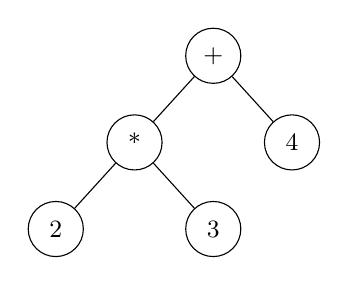
\begin{tikzpicture}[
  level distance=11mm, sibling distance=20mm, font=\small,
  every node/.style={draw,circle,inner sep=1.5pt,minimum size=7mm}
]
\node {\code{+}}
  child {node {\code{*}}
    child {node {2}}
    child {node {3}}
  }
  child {node {4}};
\end{tikzpicture}
\caption{AST de l'expression \code{2 * 3 + 4}. La priorité de \code{*} sur
\code{+} se traduit par la position des n\oe uds dans l'arbre.}
\label{fig:ast-ex}
\end{figure}

Le langage compte quatorze types de n\oe uds, recensés dans le
tableau~\ref{tab:nodetypes} avec les champs significatifs de chacun. Cette
uniformité (une seule structure \code{Node}, un champ \code{type}) est ce qui rend
les trois visiteurs, à savoir l'évaluateur, l'optimiseur et le générateur de
code, aussi réguliers à écrire.

\begin{table}[ht]
\centering
\caption{Types de n\oe uds de l'AST et champs significatifs.}
\label{tab:nodetypes}
\small
\begin{tabular}{@{}lll@{}}
\toprule
\textbf{Type} & \textbf{Rôle} & \textbf{Champs utilisés} \\
\midrule
\code{NODE\_NUM}       & littéral numérique      & \code{num} \\
\code{NODE\_VAR}       & référence de variable   & \code{name} \\
\code{NODE\_BINOP}     & opération binaire       & \code{op, left, right} \\
\code{NODE\_UNOP}      & moins unaire            & \code{op, left} \\
\code{NODE\_ASSIGN}    & affectation             & \code{name, left} \\
\code{NODE\_IF}        & conditionnelle          & \code{cond, body, elsebody} \\
\code{NODE\_WHILE}     & boucle tant que         & \code{cond, body} \\
\code{NODE\_FOR}       & boucle pour             & \code{left, cond, right, body} \\
\code{NODE\_FUNC\_DECL}& déclaration de fonction & \code{name, args, nargs, body} \\
\code{NODE\_FUNC\_CALL}& appel de fonction       & \code{name, args, nargs} \\
\code{NODE\_PRINT}     & \code{afficher}         & \code{left} \\
\code{NODE\_READ}      & \code{lire}             & aucun \\
\code{NODE\_RETURN}    & \code{retourner}        & \code{left} \\
\code{NODE\_BREAK} / \code{NODE\_CONTINUE} & ruptures de boucle & aucun \\
\code{NODE\_BLOCK}     & suite d'instructions    & \code{args, nargs} \\
\bottomrule
\end{tabular}
\end{table}

\subsection{La table des symboles}

La gestion de la portée repose sur une \textbf{pile d'environnements} (\emph{frames}),
chaque environnement étant lui-même une table de hachage. Un environnement est
empilé à l'entrée d'une fonction et dépilé à sa sortie, à l'image de la pile
d'appels matérialisée par le registre \code{\%ebp} en assembleur i386 (chapitre~2
du cours). La figure~\ref{fig:frames} illustre l'état de la pile pendant un appel
récursif.

\begin{figure}[ht]
\centering
\begin{tikzpicture}[font=\footnotesize, frame/.style={draw,minimum width=40mm,minimum height=8mm,align=center}]
  \node[frame] (g) {environnement \textbf{global} \\ \code{i = 3}};
  \node[frame,above=2mm of g] (f1) {frame \code{fib(3)} \\ \code{n = 3}};
  \node[frame,above=2mm of f1] (f2) {frame \code{fib(2)} \\ \code{n = 2}};
  \node[frame,above=2mm of f2,fill=black!8] (f3) {frame \code{fib(1)} \quad$\leftarrow$ sommet \\ \code{n = 1}};
  \draw[-{Stealth}] (f3.east) to[bend left=30] node[right,font=\scriptsize]{parent} (f2.east);
  \draw[-{Stealth}] (f2.east) to[bend left=30] (f1.east);
  \draw[-{Stealth}] (f1.east) to[bend left=30] (g.east);
\end{tikzpicture}
\caption{Pile d'environnements pendant l'évaluation de \code{fib(3)}. Le lien
\emph{parent} sert à restaurer le frame courant en sortie de fonction ; la
résolution des variables, elle, est lexicale (frame courant puis global).}
\label{fig:frames}
\end{figure}

\subsection{Algorithmes clés}

\paragraph{Évaluation.} L'évaluateur est une fonction récursive renvoyant une
\code{Value}. Son principe, pour les n\oe uds principaux, est résumé en
pseudo-code dans le listing~\ref{lst:eval-pseudo}.

\begin{lstlisting}[style=c,caption={Principe de l'évaluateur (pseudo-code).},label={lst:eval-pseudo}]
Value eval(Node n):
    selon n.type:
      NUM       -> renvoyer n.num
      VAR       -> chercher n.name dans l'environnement (erreur si absent)
      BINOP     -> a=eval(gauche); b=eval(droite); appliquer l'operateur
      ASSIGN    -> v=eval(expr); ranger v sous n.name; renvoyer v
      IF        -> si eval(cond) vrai: eval(alors) sinon: eval(sinon)
      WHILE/FOR -> boucler tant que eval(cond), en surveillant
                   les signaux retourner / arreter / continuer
      FUNC_CALL -> evaluer les args (frame appelant), empiler un frame,
                   lier les parametres, evaluer le corps, depiler
      RETURN    -> return_value=eval(expr); lever le drapeau de retour
      BLOCK     -> evaluer chaque instruction, en s'arretant des qu'un
                   signal de rupture de flot est leve
\end{lstlisting}

\paragraph{Optimisation.} L'optimiseur est un second parcours qui \emph{réécrit}
l'arbre. Deux transformations sont appliquées : le \emph{pliage de constantes}
(un n\oe ud binaire dont les deux fils sont des littéraux est remplacé par le
littéral résultat) et l'\emph{élimination du code mort} (une conditionnelle dont
la condition est un littéral est remplacée par la seule branche atteignable). Le
détail, y compris le garde-fou contre la division par zéro, est exposé au
chapitre~\ref{chap:implementation}.
